Nick Vosseteig

2014-01-16

building, wiring, destroying

\begin{tabular}{|p{5cm}|p{5cm}|}
 \hline
 building&
We rebuilt the intake device so that it now uses surgical tubing and is on a single axle. We also rebuilt the linear slides because the old ones broke.
 \\
 \hline
destroying&
We took apart a lot of the robot in order to remove the broken or temporary pieces from the competition. We plan to refabricate similar pieces with improvments and made out of polycarb.
 \\
 \hline
wiring&
Some of the wiring was messed up after the competition so we fixed it up, but some will probably still need to be changed after we add back new pieces.
 \\
 \hline
\end{tabular}

\section*{building}
Our front intake device was taking up too much space, would tip the robot up when picking up a large ball, and was not very effective at picking up balls off the walls. The new intake devices uses surgical tubing so that we could add a support beam behind it. The surgical tubing picks up balls well, and bends against the support beam allowing it to spin. Here is a picture of the new intake device:

\begin{center}
 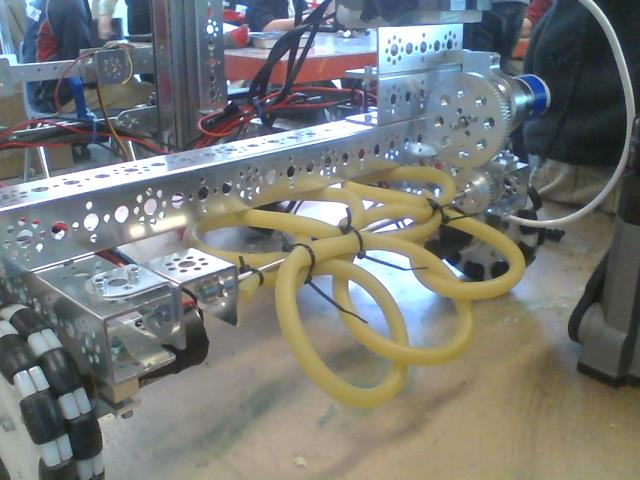
\includegraphics[width=215px]{./Entries/Images/new_intake.jpg}
\end{center}

\section*{Destroying}
The robot was put together with a lot of cardboard and some wood and tape. Because of this the robot had a lot of broken parts after the competition. We needed to remove all the temporary and broken parts so that we can work on more permanent, polycarb pieces for the next competition.
